\input{../../.preambles/01-semester_work}
\input{../../.preambles/10-russian}
\input{../../.preambles/20-math}
\input{../../.preambles/30-physics}

\newcommand{\ds}{\displaystyle}

\begin{document}
    \maketitlepage{Факультет электроники и вычислительной техники}
    {физики}{Вакуумная и газоразрядная электроника}{}{7}
    {студент группы Ф-369\\Чечеткин~И.~А.}{m}{доцент Ковтун~Д.~Г.}{m}
    \emph{1. Электрон со скоростью \( v \) влетает под углом \( \alpha \) к
    направлению вектора магнитной индукции \( \vec{B} = \vec{k}B_0 \). Через
    интервал времени, равный четверти периода циклотронной частоты, он попадает
    в область действия электростатического поля напряженностью
    \( \vec{E} = \vec{i}E_0\cos\beta + \vec{j}E_0\sin\beta + \vec{k}E_z \), а
    магнитное поле исчезает. Определить величину \( E_z \) и \( E_0 \), если
    электрон вернулся в точку влета.}
    \begin{figure}[h!]
        \center
        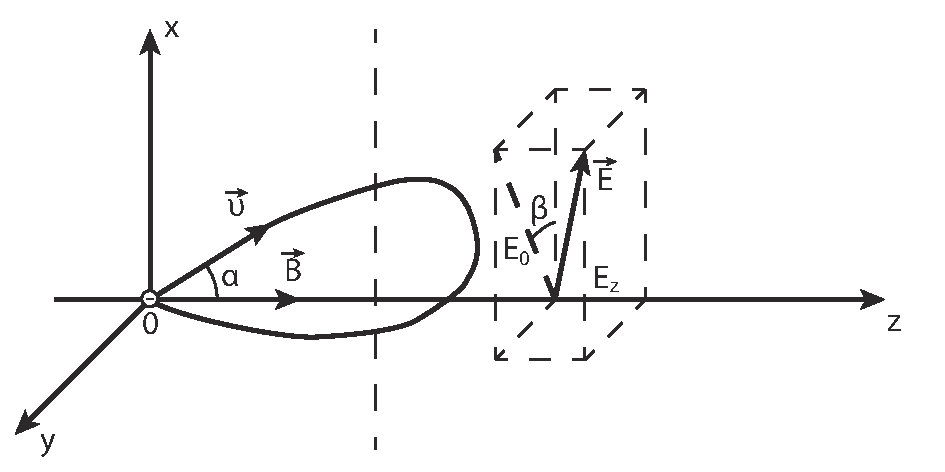
\includegraphics[width=.7\textwidth]{ch1}
    \end{figure}
    
    Запишем уравнение движение электрона в области с наведенным полем
    \( \vec{B} \) с помощью второго закона Ньютона:
    \[
        m\vec{a} = -e\vec{v}\times\vec{B} = -e
        \begin{vmatrix}
            \vec{i} & \vec{j} & \vec{k} \\
            \dot{x} & \dot{y} & \dot{z} \\
            0 & 0 & B_0
        \end{vmatrix}
        = -e\big[\vec{i}\dot{y}B_0 - \vec{j}\dot{x}B_0\big].
    \]
    Разделим обе части на массу электрона, тогда в проекциях на координатные
    оси получим:
    \begin{align}
        & \text{Ox: } \ddot{x} = -\omega_c\dot{y}, \label{eq11} \\
        & \text{Oy: } \ddot{y} = \omega_c\dot{x}, \label{eq12} \\
        & \text{Oz: } \ddot{z} = 0, \label{eq13}
    \end{align}
    где \( \omega_c = \dfrac{eB_0}{m} \) -- циклотронная частота.
    
    Интегрируя уравнение \eqref{eq13} с учетом начальных условий:
    \( \dot{z}(0) = v\cos\alpha \) и \( z(0) = 0 \), получим
    \[
        \dot{z} = v\cos\alpha, \quad z = vt\cos\alpha.
    \]
    
    Найдем \( \dot{x} \) интегрированием уравнения \eqref{eq11}:
    \[
        \dot{x} = -\omega_cy + C, \quad C = \omega_cy(0) + \dot{x}(0) =
        v\sin\alpha, \quad \dot{x} = -\omega_cy + v\sin\alpha
    \]
    и подставим ее в уравнение \eqref{eq12}:
    \[
        \ddot{y} = -\omega_c^2y + \omega_cv\sin\alpha, \text{ или }
        \ddot{y} + \omega_c^2y = \omega_cv\sin\alpha.
    \]
    
    Представим решение этого уравнения в виде суммы общего и частного решений:
    \begin{gather*}
        y = y_\text{общ} + y_\text{част}. \\
        y_\text{общ} = A\cos\omega_ct + B\sin\omega_ct, \quad
        y_\text{част} = \frac{v\sin\alpha}{\omega_c}; \\
        y = A\cos\omega_ct + B\sin\omega_ct + \frac{v}{\omega_c}\sin\alpha.
    \end{gather*}
    
    Константы \( A \) и \( B \) найдем из начальных условий:
    \begin{align*}
        & \dot{y}(0) = 0\colon \quad -\omega_cA\sin0 + \omega_cB\cos0 = 0
        \Rightarrow B = 0; \\
        & y(0) = 0\colon \quad A\cos0 + \frac{v}{\omega_c}\sin\alpha = 0
        \Rightarrow A = -\frac{v}{\omega_c}\sin\alpha.
    \end{align*}
    
    Таким образом, \( y = \dfrac{v}{\omega_c}\Big[1 - \cos\omega_ct\Big]
    \sin\alpha \), \( \dot{y} = v\sin\alpha\sin\omega_ct \).
    
    Тогда:
    \begin{gather*}
        \dot{x} = -v\sin\alpha\big[1 - \cos\omega_ct\big] + v\sin\alpha =
        v\sin\alpha\cos\omega_ct. \\
        x = \frac{v}{\omega_c}\sin\alpha\sin\omega_ct.
    \end{gather*}
    
    В момент времени \( \tau \), равный четверти периода циклотронной частоты
    \( \tau = \dfrac{1}{4}T_c = \dfrac{1}{4}\dfrac{2\pi}{\omega_c} =
    \dfrac{\pi}{2\omega_c} \):
    \begin{align*}
        \dot{x}(\tau) = v\sin\alpha\cos\frac{\pi}{2} = 0, & & &
        x(\tau) = \frac{v}{\omega_c}\sin\alpha\sin\frac{\pi}{2} =
        \frac{v}{\omega_c}\sin\alpha; \\
        \dot{y}(\tau) = v\sin\alpha\sin\frac{\pi}{2} = v\sin\alpha, & & &
        y(\tau) = \frac{v}{\omega_c}\Big[1 - \cos\frac{\pi}{2}\Big]\sin\alpha =
        \frac{v}{\omega_c}\sin\alpha; \\
        \dot{z}(\tau) = v\cos\alpha, & & &
        z(\tau) = \frac{v}{\omega_c}\frac{\pi}{2}\cos\alpha.
    \end{align*}
    
    Запишем уравнение движение электрона в области с наведенным полем
    \( \vec{E} \) с помощью второго закона Ньютона:
    \[
        m\vec{a} = -e\vec{E}.
    \]
    Разделим обе части на массу электрона, тогда в проекциях на координатные
    оси получим:
    \begin{align*}
        & \text{Ox: } \ddot{x} = -\frac{eE_0}{m}\cos\beta, \\
        & \text{Oy: } \ddot{y} = -\frac{eE_0}{m}\sin\beta, \\
        & \text{Oz: } \ddot{z} = -\frac{eE_z}{m}.
    \end{align*}
    
    Интегрируя по времени два раза и учитывая, что в качестве начальных условий
    используются значения координат и скоростей в момент времени \( \tau \),
    получим зависимости координат от времени:
    \begin{align*}
        & x = -\frac{eE_0}{2m}t^2\cos\beta + \frac{v}{\omega_c}\sin\alpha, \\
        & y = -\frac{eE_0}{2m}t^2\sin\beta + vt\sin\alpha + \frac{v}{\omega_c}
        \sin\alpha, \\
        & z = -\frac{eE_z}{2m}t^2 + vt\cos\alpha + \frac{v}{\omega_c}
        \frac{\pi}{2}\cos\alpha.
    \end{align*}
    
    По условию, электрон вернется в начальную точку за время \( T \):
    \begin{align}
        & 0 = -\frac{eE_0}{2m}T^2\cos\beta + \frac{v}{\omega_c}\sin\alpha,
        \label{eq14} \\
        & 0 = -\frac{eE_0}{2m}T^2\sin\beta + vT\sin\alpha + \frac{v}{\omega_c}
        \sin\alpha, \label{eq15} \\
        & 0 = -\frac{eE_z}{2m}T^2 + vT\cos\alpha + \frac{v}{\omega_c}
        \frac{\pi}{2}\cos\alpha. \label{eq16}
    \end{align}
    
    Из уравнения \eqref{eq14} найдем время возврата электрона \( T \):
    \[
        \frac{eE_0}{2m}T^2\cos\beta = \frac{v}{\omega_c}\sin\alpha,\ 
        T^2 = \frac{2m^2v}{e^2E_0B_0}\frac{\sin\alpha}{\cos\beta};\ 
        T = \frac{m}{e}\sqrt{\frac{2v}{E_0B_0}\frac{\sin\alpha}{\cos\beta}}.
    \]
    
    Из уравнения \eqref{eq15} найдем \( E_0 \):
    \begin{gather*}
        \frac{eE_0}{2m}\frac{m^2}{e^2}\frac{2v}{E_0B_0}\frac{\sin\beta}
        {\cos\beta}\sin\alpha = \frac{mv}{e}\sin\alpha\sqrt{\frac{2v}{E_0B_0}
        \frac{\sin\alpha}{\cos\beta}} + \frac{mv}{eB_0}\sin\alpha, \\
        \frac{\tg\beta}{B_0} = \sqrt{\frac{2v}{E_0B_0}\frac{\sin\alpha}
        {\cos\beta}} + \frac{1}{B_0}, \quad \frac{1}{B_0}\Big(\tg\beta - 1\Big)
        = \sqrt{\frac{2v}{E_0B_0}\frac{\sin\alpha}{\cos\beta}}, \\
        (\tg\beta - 1)^2 = \frac{2vB_0}{E_0}\frac{\sin\alpha}{\cos\beta}, \quad
        E_0 = \frac{2vB_0\cos\alpha}{\cos\beta(\tg\beta - 1)^2} =
        \frac{2vB_0\sin\alpha}{1 - \sin2\beta}\cos\beta.
    \end{gather*}
    
    А теперь из уравнения \eqref{eq16} найдем \( E_z \):
    \begin{gather*}
        \frac{eE_z}{2m}\frac{m^2}{e^2}\frac{2v}{E_0B_0}\frac{\sin\alpha}
        {\cos\beta} = \frac{mv}{e}\sqrt{\frac{2v}{E_0B_0}\frac{\sin\alpha}
        {\cos\beta}}\cos\alpha + \frac{\pi}{2}\frac{mv}{eB_0}\cos\alpha, \\
        E_z\tg\alpha = \sqrt{2vE_0B_0\cos\beta\sin\alpha} + \frac{\pi}{2}E_0
        \cos\beta,\\
        E_z = \sqrt{\frac{2vE_0B_0\cos\beta\cos^2\alpha}
        {\sin\alpha}} + \frac{\pi E_0\cos\beta\cos\alpha}{2\sin\alpha}; \\
        E_z = \frac{2vB_0\cos\beta\cos\alpha}{\sqrt{1 - \sin2\beta}}\left(
        1 + \frac{\pi\cos\beta}{2\sqrt{1 - \sin2\beta}}\right).
    \end{gather*}
    
    \newpage
    \emph{2. Сходящийся электронный поток эмитируется с торца цилиндрического
    катода радиуса \( R_\text{к} \) с начальной скоростью \( u \) и ускоряется
    под действием напряжения \( U_0 \) первого анода электронного прожектора,
    расположенного на расстоянии \( a \) от катода. Электроны вылетают под
    углами, определяемыми образующими конуса, вершина которого лежит на
    расстоянии \( 6a \) от катода. За анодом поток летит в продольном
    фокусирующем магнитном поле с величиной магнитной индукции \( B_0 \).
    Считая, что с катода снимается ток величиной \( I_\text{к} \), определить:
    период пульсаций, максимальный радиус электронного потока. Считать, что
    распределение поля между катодом и первым анодом эквивалентно распределению
    поля между двумя параллельными плоскостями.}
    \begin{figure}[h!]
        \center
        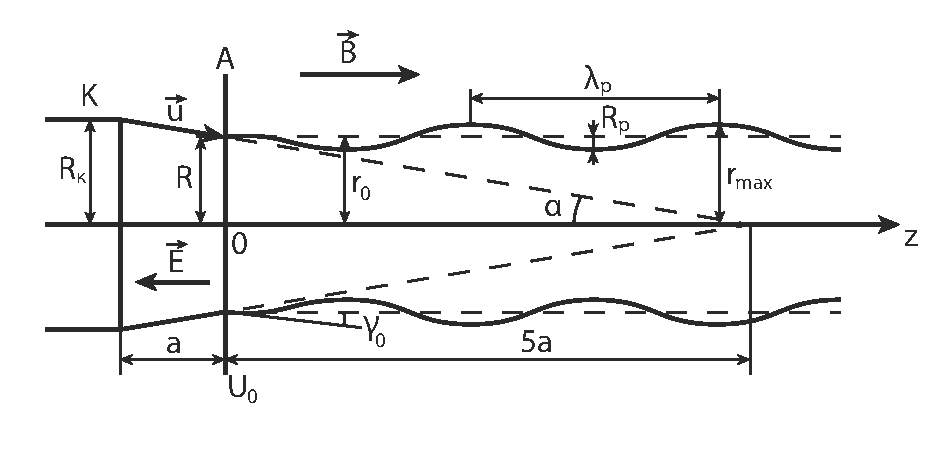
\includegraphics[width=.7\textwidth]{ch2}
    \end{figure}
    
    Запишем уравнение движения электрона потока в области между катодом и
    первым анодом:
    \[
        m\vec{a} = -e\vec{E},\ \vec{a} = -\frac{e}{m}\vec{E},\ 
        \vec{E} = -\frac{U_0}{a}\vec{k}.
    \]
    
    В цилиндрических координатах, с учетом того, что \( \dot{\phi} = 0 \):
    \[
        \ddot{r} = 0, \quad \ddot{z} = \frac{e}{m}\frac{U_0}{a}.
    \]
    
    Для крайнего электрона потока: \( \dot{r}(0) = -u\sin\alpha \),
    \( r(0) = R_\text{к} \), \( \dot{z}(0) = u\cos\alpha \), \( z(0) = -a \),
    \( \alpha = \arctg\dfrac{R_\text{к}}{6a} \). Интегрируя уравнение движения
    с такими начальными условиями, получим:
    \[
        \dot{r} = -u\sin\alpha,\ r = -ut\sin\alpha + R_\text{к}, \quad
        \dot{z} = \frac{e}{m}\frac{U_0}{a}t + u\cos\alpha,\ 
        z = \frac{e}{m}\frac{U_0}{a}\frac{t^2}{2} + ut\cos\alpha - a.
    \]
    
    Из последнего уравнения найдем время пролета области <<катод-анод>>:
    
    \[
        \frac{e}{m}\frac{U_0}{a}\frac{\tau^2}{2} + u\tau\cos\alpha - a = 0, \quad
        \tau = -\frac{amu\cos\alpha}{eU_0} + \sqrt{\left(\frac{amu\cos\alpha}
        {eU_0}\right)^2 - \frac{2a^2m}{eU_0}}.
    \]
    
    Тогда в момент \( \tau \):
    \begin{gather*}
        \dot{z}(\tau) = \sqrt{u^2\cos^2\alpha - 2\frac{eU_0}{m}} = v_0, \\
        r(\tau) = R_\text{к} + \frac{amu^2\cos\alpha\sin\alpha}{eU_0} -
        u\sin\alpha\sqrt{\left(\frac{amu\cos\alpha}{eU_0}\right)^2 -
        \frac{2a^2m}{eU_0}} = R.
    \end{gather*}
    
    Запишем уравнение движения электрона потока в области за анодом:
    \[
        m\vec{a} = -e\vec{E}_\text{пр} - e\vec{v}\times\vec{B},\quad
        \vec{v} \times \vec{B} =
        \begin{vmatrix}
            \vec{e}_r & \vec{e}_\phi & \vec{e}_z \\
            \dot{r} & r\dot{\phi} & \dot{z} \\
            0 & 0 & B_0 
        \end{vmatrix}
        = \vec{e}_r\big(r\dot\phi B_0\big) - \vec{e}_\phi\big(\dot{r}B_0\big).
    \]
    
    В проекциях на оси координат:
    \begin{equation}
        \left\{ \begin{array}{l}
            \ds \ddot{r} - r(\dot{\phi})^2 = -\frac{e}{m}E_r - \frac{e}{m}B_0r
            \dot{\phi}, \\
            \ds \frac{1}{r}\der{}{t}\big(r^2\dot{\phi}\big) = \frac{e}{m}B_0
            \dot{r},
        \end{array} \right. \quad \text{где }
        E_r = -\frac{I_\text{к}}{2\pi\Ezero v_0r}.
        \label{eq21}
    \end{equation}
    
    Поток вектора \( \vec{B} \) через поверхность круга радиуса \( r \):
    \[
        \psi(r, z) = 2\pi\int\limits_0^r B_0r\,dr = 2\pi B_0\frac{r^2}{2} =
        \pi r^2B_0.
    \]
    Тогда \( \dot\psi \):
    \[
        \dot{\psi} = \pder{\psi}{t} = \pder{\psi}{r}\pder{r}{t} + \pder{\psi}
        {z}\pder{z}{t} = 2\pi rB_0\pder{r}{t} = 2\pi rB_0\dot{r}.
    \]
    
    Распишем второе уравнение системы \eqref{eq21}:
    \[
        \frac{1}{r}\der{}{t}\big(r^2\dot\phi\big) = \frac{e}{m}B_0\dot{r},\ 
        \der{}{t}\big(r^2\dot\phi\big) = \frac{e}{m}B_0r\dot{r},\ 
        \der{}{t}\big(r^2\dot\phi\big) = \frac{\psi}{2\pi}\frac{e}{m}.
    \]
    
    Интегрируем, учитывая начальные условия \( r(\tau) = R \),
    \( \dot{\phi}(\tau) = 0 \), \( \psi\Big|_{t = \tau} = 0 \):
    
    \[
        r^2\dot\phi = \frac{e\psi}{2\pi m} = \frac{e}{2\pi m}\pi r^2B_0, \quad
        \dot\phi = \frac{eB_0}{2m} = \frac{\omega_c}{2}.
    \]
    
    Подставляя значение \( \dot\phi \) в первое уравнение системы \eqref{eq21}:
    \[
        \ddot{r} - r\frac{\omega_c^2}{4} = \frac{eI_\text{к}}{2\pi\Ezero v_0rm}
        - r\frac{\omega_c^2}{2}, \quad \ddot{r} + r\frac{\omega_c^2}{4}
        - \frac{eI_\text{к}}{2\pi\Ezero v_0rm} = 0.
    \]
    
    Перейдем к уравнению траектории \( r(z) \) \( \Big(\ds \ddot{r} =
    \dder{r}{z}v_0\Big) \):
    \begin{gather*}
        \ppder{r}{z} + \frac{r\omega_c^2}{4v_0^2} - \frac{eI_\text{к}}
        {2\pi\Ezero v_0^3rm} = 0.
    \end{gather*}

    При некотором равновесном радиусе \( \ds r_0^2 = \frac{4v_0^2eI_\text{к}}
    {2\pi\Ezero v_0^3m\omega_c^2} = \frac{2eI_\text{к}}{m\omega_c^2\Ezero v_0
    \pi} \) ускорение по радиусу будет отсутствовать, и электронный поток будет
    сохранять свою форму, то есть будет бриллюэновским.
    
    Пусть поток отклоняется от равновесного радиуса \( r_0 \) на некоторую
    величину \( \delta \ll 1 \): \( r = r_0(1 + \delta) \).
    
    Учитывая разложение \( \ds \frac{1}{r} = \frac{1}{r_0}\big(1 -
    \delta\big) \), получим дифференциальное уравнение относительно
    \( \delta \):
    \[
        \dder{}{z}\Big[r_0(1 + \delta)\Big] + \frac{r_0(1 + \delta)\omega_c^2}
        {4v_0^2} - \frac{eI_\text{к}}{2\pi\Ezero v_0^3r_0m}\Big(1 - \delta\Big)
        = 0, \quad
        \dder{\delta}{z} + \frac{\omega_c^2}{2v_0^2}\delta = 0.
    \]
    
    Обозначая \( \alpha^2 = \dfrac{\omega_c^2}{2v_0^2} \), тогда
    \( \ds\dder{\delta}{z} + \alpha^2\delta = 0 \).
    
    Решение этого уравнения \( \delta = D\cos(\alpha z + \beta) \).
    
    Из начальных условий \( \ds\delta(0) = \frac{R}{r_0}\left(1 - \frac{r_0}{R}
    \right) \), \( \delta'(0) = \dfrac{\tg\gamma_0}{r_0} \) найдем \( D \) и
    \( \beta \):
    \begin{gather*}
        D = \sqrt{\delta^2(0) + \left(\frac{\delta'(0)}{\alpha}\right)^2} =
        \frac{R}{r_0}\sqrt{\left(1 - \frac{r_0}{R}\right)^2 + 2\left(\frac{\tg
        \gamma_0v_0}{\omega_cR}\right)^2}; \\
        \beta = -\arctg\left(\frac{\delta'(0)}{\alpha\delta(0)}\right) =
        -\arctg\left(\frac{\sqrt{2}v_0\tg\gamma_0}{\left(1 - \frac{r_0}{R}
        \right)R\omega_c}\right) \text{ -- начальная фаза пульсаций.}
    \end{gather*}
    
    Радиус пульсаций: \( R_p = r_0D \). Длина волны пульсаций: \( \ds\lambda_p
    = \frac{2\pi}{\alpha} = \frac{\sqrt{8}\pi v_0}{\omega_c} \). Период
    пульсаций: \( \ds T_p = \frac{\lambda_p}{c} = \frac{\sqrt{8}\pi v_0}
    {\omega_cc} \). Максимальный радиус пучка:
    
    \[
        r_{max} = r_0 + R_p = r_0\left(1 + R\sqrt{\left(1 - \frac{r_0}{R}
        \right)^2 + 2\left(\frac{\tg\gamma_0v_0}{\omega_cR}\right)^2}\right).
    \]
\end{document}
